\subsection{Model}
\begin{frame}{Markov chain model}
\paragraph{Modelling dependence between time step :}
If an animal is feeding at time $i$, he has more chance to be feeding at time $i+1$ than if he was travelling at time $i$.
$$P(Z_{i+1}=1 \vert Z_{i}=1) \ne P(Z_{i+1}=1 \vert Z_{i}=2)$$

\paragraph{Markov Chain definition}
$\Zbf$ is a Markov chain if 
$$P(Z_{i+1} \vert Z_{1:i}) =  P(Z_{i+1} \vert Z_{i})$$


$\Zbf$ is completely defined by the distribution $\mu_1=P(Z_1)$ and the transition matrix
$$\Pi =\left[\begin{matrix}
\pi_{11} & 1-\pi_{11}\\
1-\pi_{22} & 1-\pi_{22}
\end{matrix}\right]$$
\end{frame}

\begin{frame}[fragile]{Markov chain simulation}

\begin{columns}
\begin{column}{0.5\textwidth}
\begin{knitrout}
\definecolor{shadecolor}{rgb}{0.969, 0.969, 0.969}\color{fgcolor}\begin{kframe}
\begin{alltt}
\hlcom{### Hidden State simulation}
\hlstd{N} \hlkwb{<-} \hlnum{200}
\hlstd{pi11} \hlkwb{<-} \hlnum{0.8}
\hlstd{pi22} \hlkwb{<-} \hlnum{0.9}
\hlcom{## initial distribution}
\hlstd{mu1} \hlkwb{<-} \hlkwd{c}\hlstd{(}\hlnum{0.5}\hlstd{,} \hlnum{0.5}\hlstd{)}
\hlcom{##transition matrix}
\hlstd{PI} \hlkwb{<-} \hlkwd{matrix}\hlstd{(}\hlkwd{c}\hlstd{(pi11,} \hlnum{1}\hlopt{-}\hlstd{pi11,} \hlnum{1}\hlopt{-}\hlstd{pi22, pi22),} \hlkwc{ncol}\hlstd{=}\hlnum{2}\hlstd{,} \hlkwc{byrow} \hlstd{= T)}

\hlcom{##initialisation of Z}
\hlstd{Z} \hlkwb{<-} \hlkwd{rep}\hlstd{(}\hlnum{NA}\hlstd{, N)}
\hlstd{Z[}\hlnum{1}\hlstd{]} \hlkwb{<-} \hlkwd{sample}\hlstd{(}\hlnum{1}\hlopt{:}\hlnum{2}\hlstd{,} \hlkwc{size}\hlstd{=}\hlnum{1}\hlstd{,} \hlkwc{prob} \hlstd{= mu1)}
\hlkwa{for}\hlstd{( i} \hlkwa{in} \hlnum{1}\hlopt{:}\hlstd{(N}\hlopt{-}\hlnum{1}\hlstd{))}
\hlstd{\{}
  \hlstd{Z[i}\hlopt{+}\hlnum{1}\hlstd{]} \hlkwb{<-} \hlkwd{sample}\hlstd{(}\hlnum{1}\hlopt{:}\hlnum{2}\hlstd{,} \hlkwc{size}\hlstd{=}\hlnum{1}\hlstd{,} \hlkwc{prob} \hlstd{= PI[Z[i],])}
\hlstd{\}}
\hlkwd{plot}\hlstd{(}\hlnum{1}\hlopt{:}\hlstd{N, Z,} \hlstr{"s"}\hlstd{)}
\hlkwd{points}\hlstd{(}\hlnum{1}\hlopt{:}\hlstd{N, Z,} \hlkwc{col}\hlstd{=Z}\hlopt{+}\hlnum{1}\hlstd{,} \hlkwc{pch}\hlstd{=}\hlnum{19}\hlstd{)}
\end{alltt}
\end{kframe}
\end{knitrout}
\end{column}
\begin{column}{0.4\textwidth}
\includegraphics[scale=0.3]{hmmCode1-1.pdf}
\end{column}
\end{columns}
\end{frame}

\begin{frame}[fragile]{Hidden Markov Chain model}
\paragraph{Model}
For a given number of states $K$, 
\begin{itemize}
\item
 \blue{Hidden States $\Zbf$ model}: $\Zbf$ is assumed to follow a Markov Chain model with unknown initial distribution $\mubf$ and transition matrix  $\Pibf$.
 \item \blue{Observations $\Ybf$ model}: The $Y_i's$ are assumed to be independent  conditionnaly to $\Zbf$ : $(Y_i\vert Z_i = k) \overset{i.i.d}{\sim} f_{\theta_k}().$
\end{itemize}
 \onslide<2->{\centering{\blue{Model parameters are $\mubf$, $\Pibf$ and $\thetabf$}}\par}
 \onslide<3->{\centering{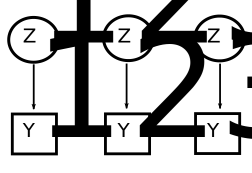
\includegraphics[scale=0.4]{Dag3.pdf}}}
\end{frame}

\begin{frame}[fragile]{Hidden Markov Chain simulation}
\begin{columns}
\begin{column}{0.5\textwidth}
\begin{knitrout}
\definecolor{shadecolor}{rgb}{0.969, 0.969, 0.969}\color{fgcolor}\begin{kframe}
\begin{alltt}
\hlcom{### observation simulation}
\hlstd{mu} \hlkwb{<-} \hlkwd{c}\hlstd{(}\hlnum{3}\hlstd{,} \hlnum{7}\hlstd{)}
\hlstd{sigma} \hlkwb{<-} \hlkwd{c}\hlstd{(}\hlnum{1}\hlstd{,}\hlnum{1.5}\hlstd{)}
\hlstd{Y.mixture} \hlkwb{<-} \hlkwd{rnorm}\hlstd{(N,} \hlkwc{mean}\hlstd{=mu[Z],} \hlkwc{sd}\hlstd{=sigma[Z])}
\hlkwd{plot}\hlstd{(Y.mixture,} \hlkwc{pch}\hlstd{=}\hlnum{19}\hlstd{)}
\hlkwd{plot}\hlstd{(Y.mixture,} \hlkwc{pch}\hlstd{=}\hlnum{19}\hlstd{,} \hlkwc{col}\hlstd{=Z}\hlopt{+}\hlnum{1}\hlstd{)}
\end{alltt}
\end{kframe}
\end{knitrout}
\end{column}
\begin{column}{0.4\textwidth}
\only<2>{\includegraphics[scale=0.3]{hmmCode2-1.pdf}}
\only<3->{\includegraphics[scale=0.3]{hmmCode2-2.pdf}}
\end{column}
\end{columns}
\end{frame}


\subsection{Parameter estimation}
%%-----------------------------------------------------------------%%
%%-----------------------------------------------------------------%%


\begin{frame}{Statistical inference of incomplete data models} 
 \paragraph{Maximum likelihood estimate:} We are looking for
  $$
  (\widehat{\thetabf},\widehat{\Pibf}, \widehat{\mubf}) = \arg\max_{\thetabf, \Pibf, {\mubf}} \log P(\Ybf; \thetabf, \Pibf, \mubf)
$$
\only<1>{
    \begin{eqnarray*}
     \log P(\Xbf, \Zbf) & = & \hid{\sum_k Z_{1k} \log \nu_k }\\
     & &\hid{+ \sum_{i > 1} \sum_{k, \ell}
       Z_{i-1,k}Z_{i,\ell} \log \pi_{k\ell}} \\
     & & + \obsy{\sum_i \sum_k Z_{ik} \log f(X_i ; \gamma_k)} 
  \end{eqnarray*}
}
\only<2>{
  \begin{eqnarray*}
    \Esp\left( \log P(\Xbf, \Zbf)\vert Y_{1:N}\right)  & = & \Ehid{\sum_k\Esp\left( Z_{1k} \vert Y_{1:N}\right) \log \nu_k }\\
     & &\Ehid{+ \sum_{i > 1} \sum_{k, \ell}
      \Esp\left( Z_{i-1,k}Z_{i,\ell}\vert Y_{1:N}\right) \log \pi_{k\ell}} \\
     & & + \Eobsy{\sum_i \sum_k \Esp\left(Z_{ik}\vert Y_{1:N}\right) \log f(X_i ; \gamma_k)} 
  \end{eqnarray*}
}
\only<3>{
  \begin{eqnarray*}
   \Esp\left(  \log P(\Xbf, \Zbf) \vert Y_{1:N}\right) & = & \Ehid{\sum_k\P\left( Z_{1}=k \vert Y_{1:N}\right) \log \nu_k }\\
     & &\Ehid{+ \sum_{i > 1} \sum_{k, \ell}
      \P\left( Z_{i-1}=k, Z_{i}=l\vert Y_{1:N}\right) \log \pi_{k\ell}} \\
    & & + \Eobsy{\sum_i \sum_k \P \left( Z_{i}=k\vert Y_{1:N}\right) 
    \log f(X_i ; \gamma_k)}
  \end{eqnarray*}
}
\end{frame}

 
\frame{ \frametitle{EM Algorithm (Baum Welch)}
  \begin{itemize}
  \item Initialisation of $\thetabf^{(0)}=(\Pi, \gamma_1, ..., \gamma_K)^{(0)}$.
  \item While the convergence is not reached 
  \end{itemize}   
 \begin{description}
    \item[E-step] Calculation of 
      \begin{eqnarray*}
        \tau^{(\ell)}_{ik}&=&P(Z_i = k | Y_{1:n}, \thetabf^{(\ell-1)})\\
        \eta_{ikh}^{(\ell)} &=& \Esp[Z_{i-1,k}Z_{ih}| Y_{1:n}, \thetabf^{(\ell-1)}]\\
      \end{eqnarray*}
    \item[M-step] Maximization in $\thetabf=(\pibf, \gammabf)$ of
    \end{description} 
 $$
 \sum_k \tau^{(\ell)}_{1k}\log \nu_k
 + \sum_{i > 1} \sum_{k, h} \eta_{ikh}^{(\ell)} \log \pi_{kh}
 + \sum_i \sum_k \tau^{(\ell)}_{ik} \log f(x_i; \gamma_k) 
 $$
 }
\begin{frame}{Reconstruction of hidden state $\Zbf$}
\paragraph{Most credible value for $Z_i$:}
We are interested in 
$$\argmax_{k}\P(Z_i= k \vert Y_{1:n})=\argmax_k \tau_{ik}.$$
\pause
\paragraph{Most credible sequence for $\Zbf$}
We are interested in 
$$\argmax_{k_1, \ldots k_n}\P(Z_1= k_1, \ldots Z_n=k_n \vert Y_{1:n})= ???$$
\pause
But force brut algorithm is not possible 
$$\longrightarrow \mbox{a smart algorithm : Viterbi algorithm}$$
\end{frame}
